\documentclass[a4paper,11pt,titlepage]{article}
\usepackage{graphicx}
\author{Abrie Greeff\\B.Sc Hons (Computer Science)\\Department of Computer Science\\University of Stellenbosch}
\title{Generating Pseudo Random Numbers}
\begin{document}
\maketitle
\tableofcontents
\section{Introduction}
Random numbers are a set of numbers that have no relation to each other. This means that for every number chosen in a set of numbers the probability is the same that any other number in the set could have been chosen. This property of random numbers is what makes it so useful. A lot of scientific fields and other non-scientific fields use this property to develop models to describe problems.\\
There are two main types of random numbers. The first is a truly random number and the other is a pseudo random number. Truly random numbers are numbers that are totally random sets. A example of truly random numbers would be if a person was asked to pick ten numbers from a list. Those ten numbers will almost always differ between each person. This kind of behaviour is exactly the behaviour anyone who is developing some kind of model would want. The first problem with truly random numbers now become evident, "How does a computer generate truly random numbers?" \\
At the time of writing no known method has been developed that can generate truly random numbers. However there has been methods developed that \emph{simulate} truly random numbers. These are called pseudo random numbers. There are two main classes of pseudo random number generating algorithms. These are the Linear Congruency Generator (LCG) algorithm and the Tausworthe algorithm.\\
LCG algorithms define a function where each newly generated number is calculated from the previous number. This function is\\
$X_i = (aX_{i-1}+b)$ \emph{mod} m\\
, where the choices of a, $X_0$, b and m are critical in the results of the function.	When good values are chosen this function gives very good output. This report focuses on the second algorithm, the Tausworthe algorithm.
\section {Tausworthe Pseudo Random Numbers}
The Tausworthe algorithm looks at every number it generates in binary format. When the next number must be generated a set of binary operations are performed on the current number to compute the next one. The main binary operation used is the exclusive-or (XOR) of bits. The XOR operation, $\oplus$, is defined as,
\\\\
$
x = \left\{ \begin{array}{ll}
0 &  ,0 \oplus 0\\
0 &  ,1 \oplus 1\\
1 &  ,0 \oplus 1
\end{array}\right.
$
\\\\
The problem is defining a set of binary operations that give a good set of random numbers. In the following sections I will concentrate on different operations I used to obtain a good set of random numbers.
\section{Implementation}
The algorithm was implemented in Java version 1.5. I used the \emph{BitSet} class to store the number instead of using one variable. This gave me the option of generating very large numbers without being constrained by the amount of bits a variable can store.

The program asks for a limit of how many numbers must be generated. The algorithm is then looped continuously until this limit is reached. The algorithm starts with a initial number called a seed on the first iteration. Every time a new number must be generated the previous generated number is the new seed. The binary operations is performed on the seed until the limit is reached.

I considered three sets of binary operations for my program. The first one was ,
\\\\
$a_i(t+1)=a_{i-1}(t) \oplus (a_i(t) \textrm{ AND } a_{i+1}(t))$
\\\\
, where \emph{i} indexes bit \emph{i} in the seed. The seed was considered to be circular, which means when the first bit or last bit was reached they could index on opposites sides. The second algorithm was,
\\\\
$a_i(t+1)=a_{i-1}(t) \oplus (a_i(t) \textrm{ AND NOT } a_{i+1}(t))$
\\\\
The first two algorithms I used were defined in [1]. The last algorithm was one I created on my own. Instead of working with individual bits the whole number was used. This algorithm is as follows,
\\\\
seed(t+1) = (seed(t) $>>>$ 15 bits) $\oplus$ (seed(t) $<<<$  11 bits) $\oplus$ (seed(t))
\\\\
, where $>>>$ is defined as rotate bits right and $<<<$ rotate bits left.
When either of these algorithms generate a new number it is written to disk in binary and decimal format. To test the numbers I generated another two programs were developed. These subsections describe them in more detail.
\subsection{Plotting program}
The plotting program's main function is the plotting of the numbers. Two different types of plots were implemented. The first one, the dotplot, goes through the numbers and plots them on the screen against each other. Two numbers were read at a time. One number was the \emph{x} point and the other the \emph{y} point on the axis. This enabled a good view of any discernable patterns that may be occurring when the numbers are generated. The second one was a frequency plot that enabled me to see which numbers were occurring more frequently.
The plot program has one further function, the checking of which numbers were not generated in the possible range of numbers. These numbers are displayed as well as what percentage of the total numbers they represent.
\subsection{Runs up test program}
The runs up test program is based on an algorithm obtained from [1]. This is a statistical test program to test for any patterns that may be occurring. I didn't use this program because the results my plot program gave was much more conclusive.
\section{Testing}
The first test I did was to determine which of the three functions gave the best results. The first two gave me results which were not satisfactory. The functions depended too much on the seed that was chosen and if the wrong seed was chosen a loop between two numbers occurred. The third function however gave me excellent results. When the function was plotted using my plot program no discernable patterns could be seen. I tested two cases much more than any other. These were generating 8-bit numbers and 16-bit numbers.
\subsection{8-bit Numbers}
8-bit numbers are in the range of 0 to 255. I tested when generating 256 numbers how many would be generated and found that on average 66\% of the numbers in the range were generated. When 512 numbers were generated 90\% of the numbers were generated. As more numbers were generated this increased until all the numbers were generated. The following figures give the dotplot of 8-bit numbers with a seed of 15 and a limit of 100000 numbers in different states of plotting. The frequency plot is also given in fig. 5.

\begin{figure}[htbp]
   \centering
   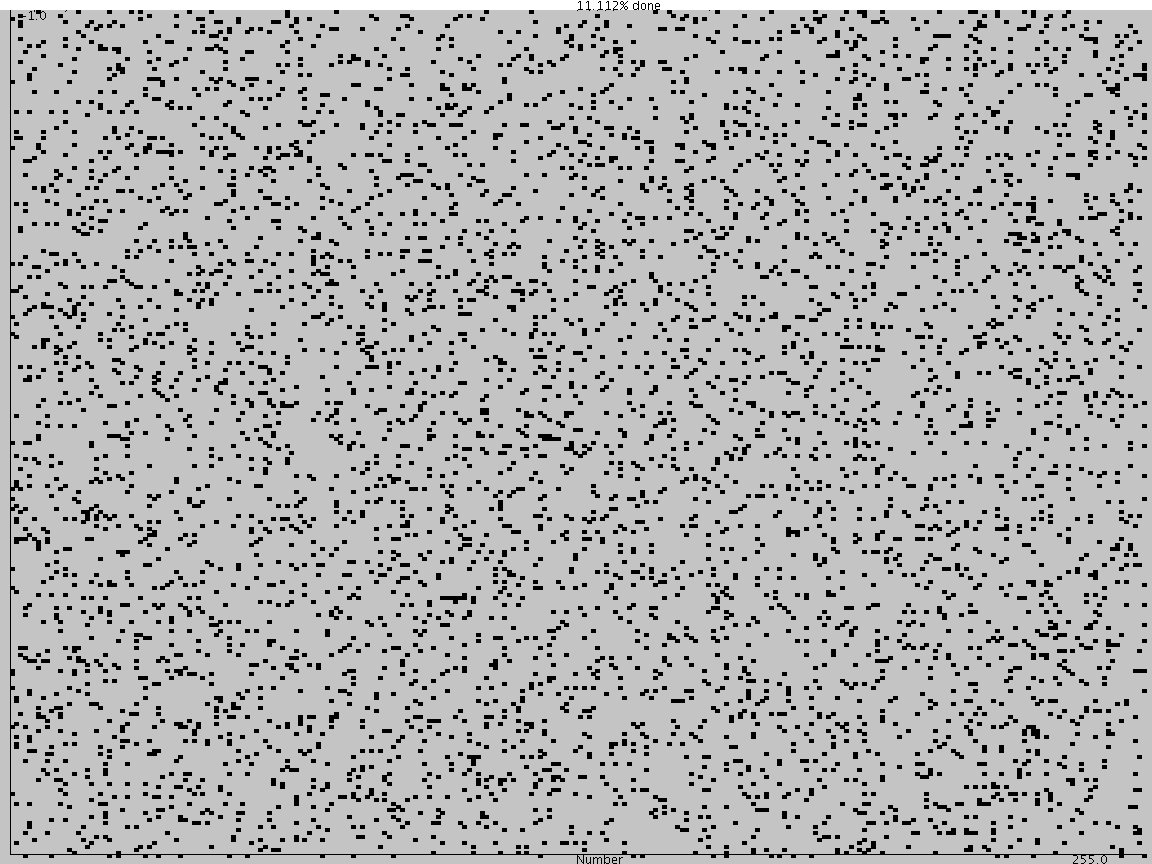
\includegraphics[width=10cm]{snapshot7.png}
   \caption{8-bit at 10\%}
   \label{Figure:figex}
\end{figure}
\begin{figure}[htbp]
   \centering
   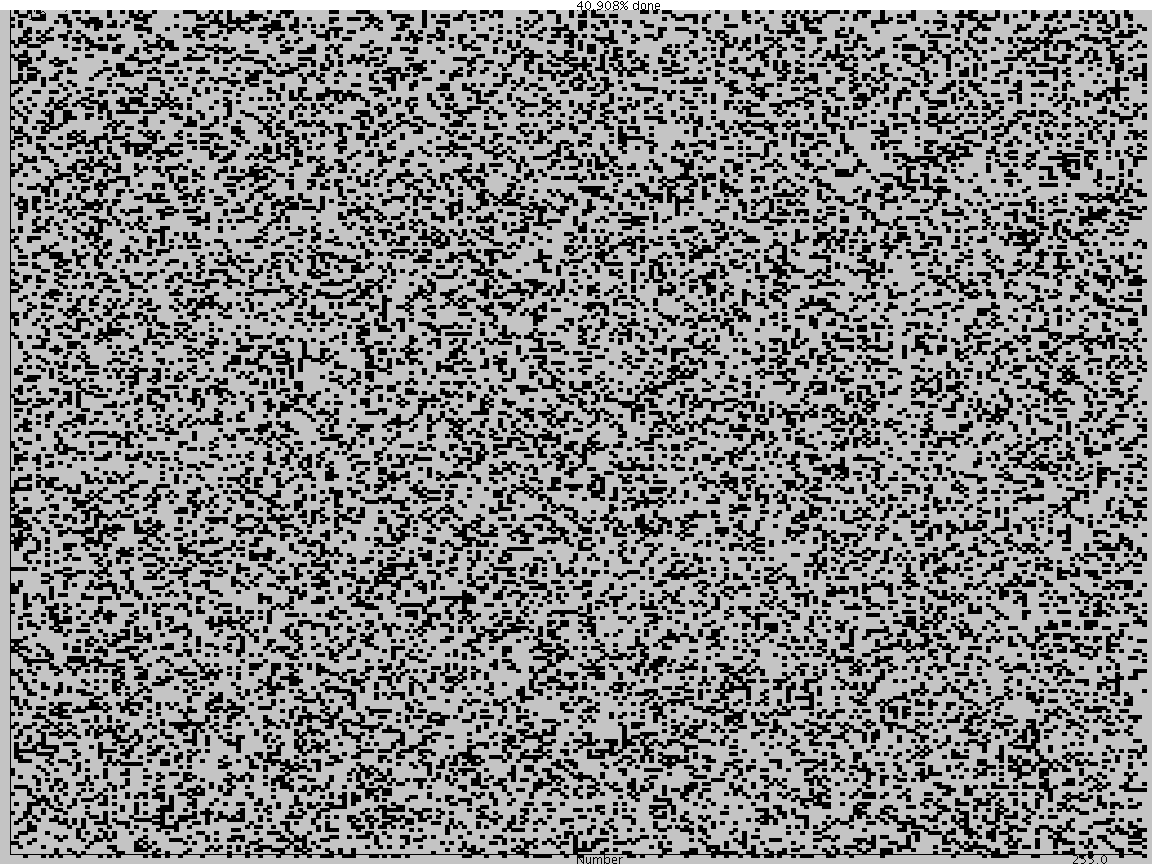
\includegraphics[width=10cm]{snapshot8.png}
   \caption{8-bit at 40\%}
   \label{Figure:figex}
\end{figure}
\begin{figure}[htbp]
   \centering
   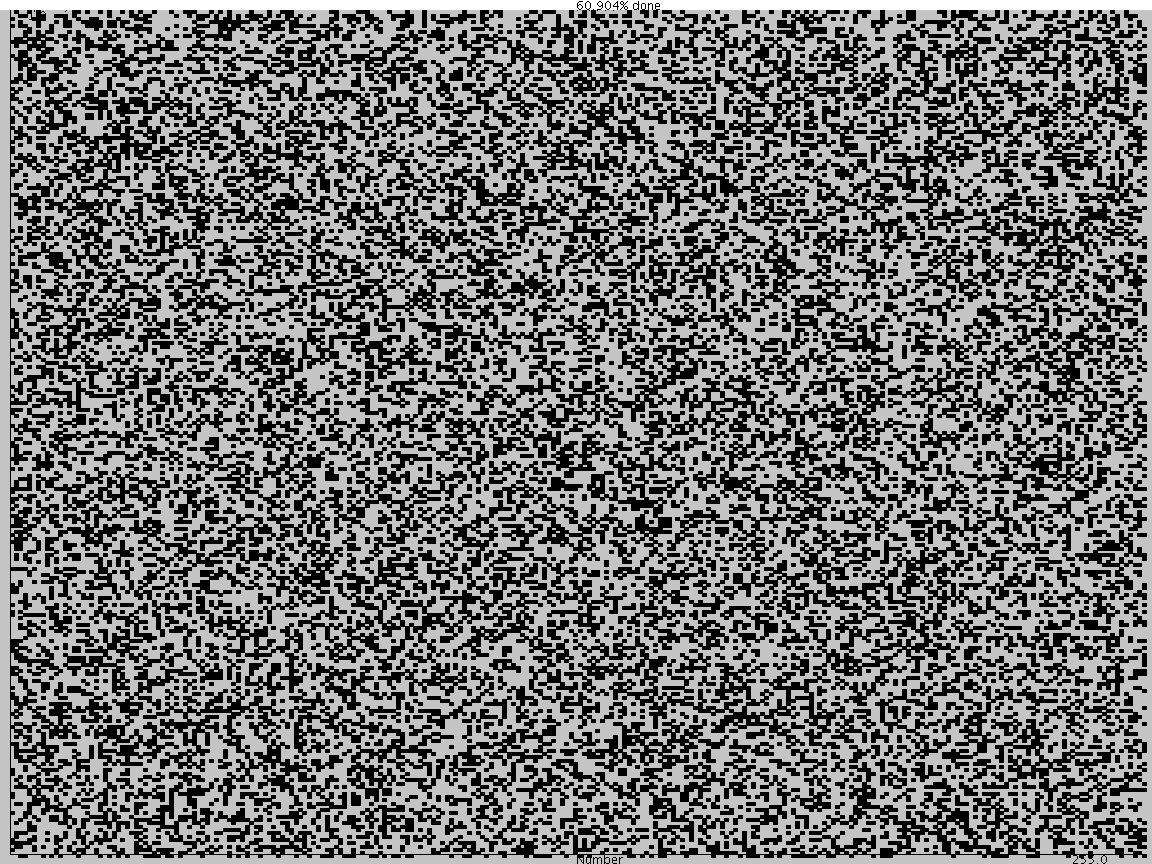
\includegraphics[width=10cm]{snapshot9.png}
   \caption{8-bit at 60\%}
   \label{Figure:figex}
\end{figure}
\begin{figure}[htbp]
   \centering
   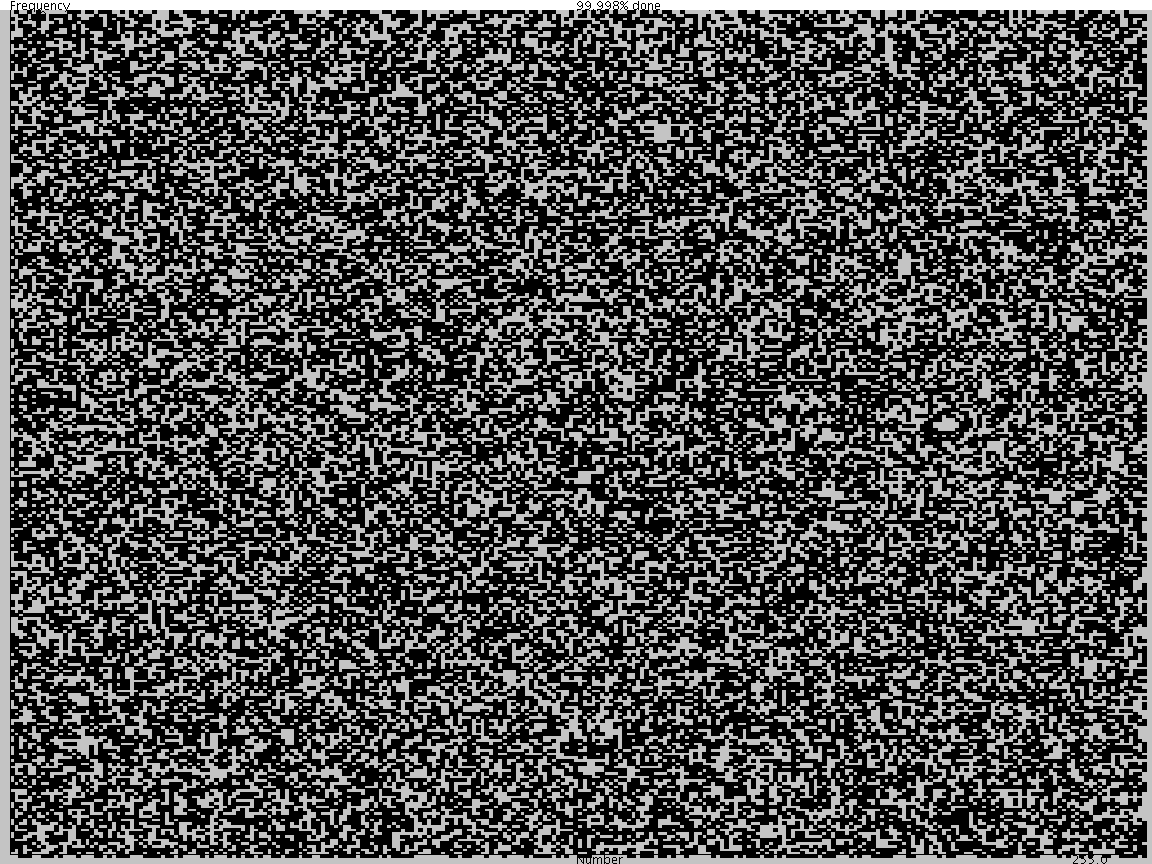
\includegraphics[width=10cm]{snapshot10.png}
   \caption{16-bit at 100\%}
   \label{Figure:figex}
\end{figure}
\begin{figure}[htbp]
   \centering
   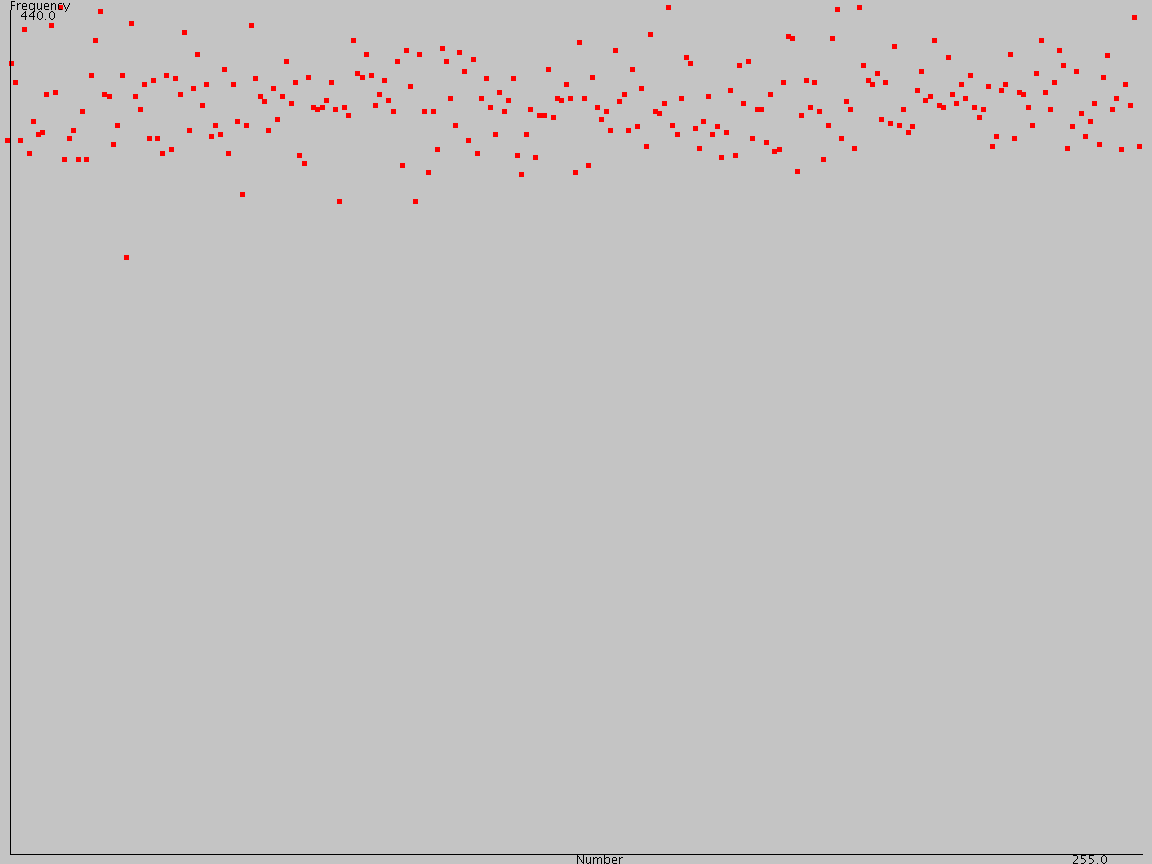
\includegraphics[width=10cm]{snapshot11.png}
   \caption{Frequency plot}
   \label{Figure:figex}
\end{figure}
\newpage
\subsection{16-bit Numbers}
16-bit numbers are in the range 0 to 65535. The same tests were performed as with 8-bit numbers. When 65536 numbers were generated 71\% numbers were generated in the range. With 120000 numbers 92\% were generated. Once again this improved until all the numbers were generated. The following figures give the dotplot of 16-bit numbers with a seed of 15 and limit of 1000000 numbers at different stages of plotting. As can be seen from the figures my function generate excellent random numbers.
\begin{figure}[htbp]
   \centering
   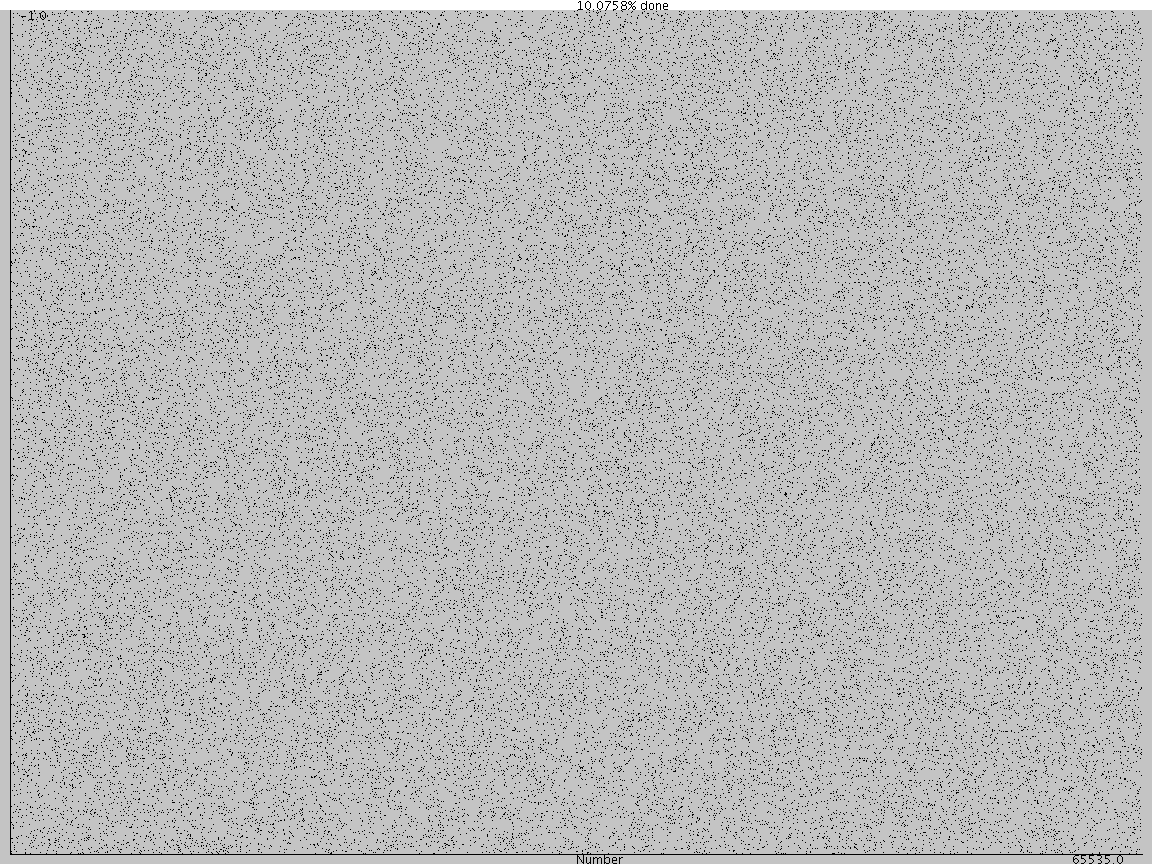
\includegraphics[width=10cm]{snapshot1.png}
   \caption{16-bit at 10\%}
   \label{Figure:figex}
\end{figure}
\begin{figure}[htbp]
   \centering
   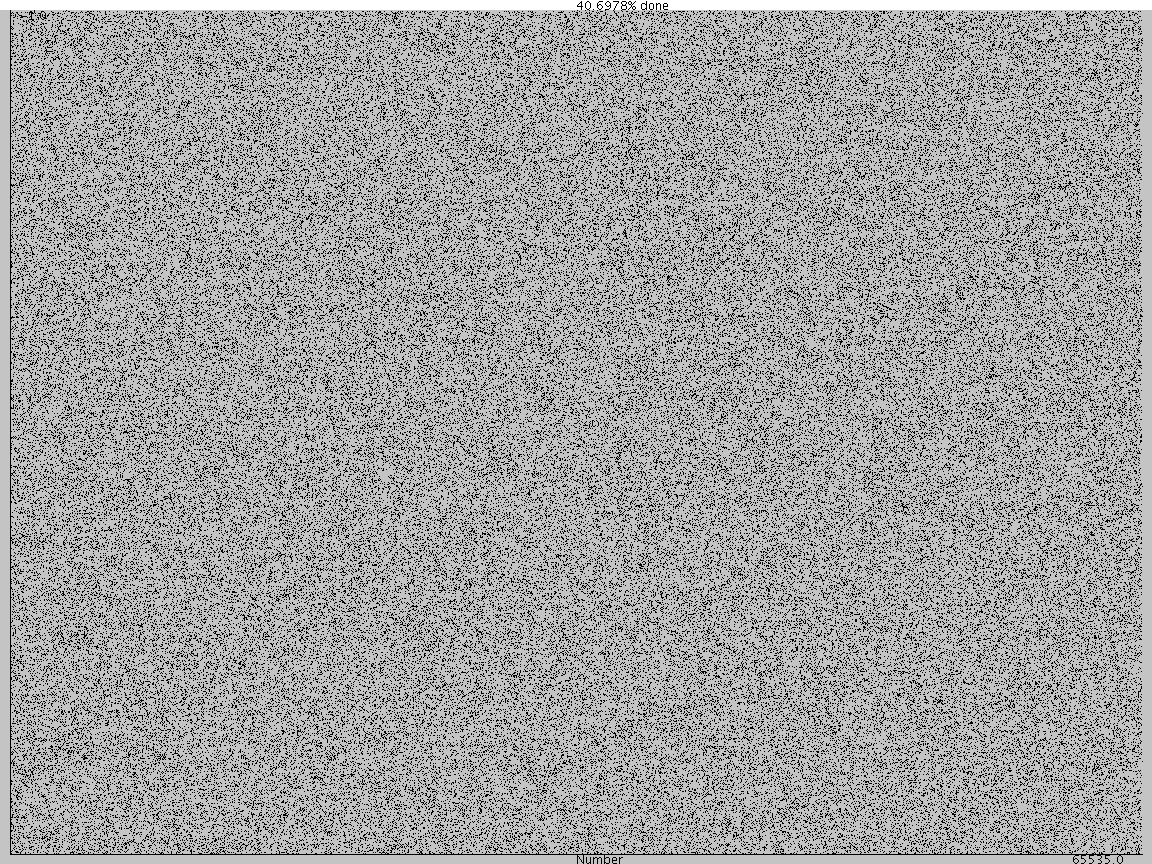
\includegraphics[width=10cm]{snapshot4.png}
   \caption{16-bit at 40\%}
   \label{Figure:figex}
\end{figure}
\begin{figure}[htbp]
   \centering
   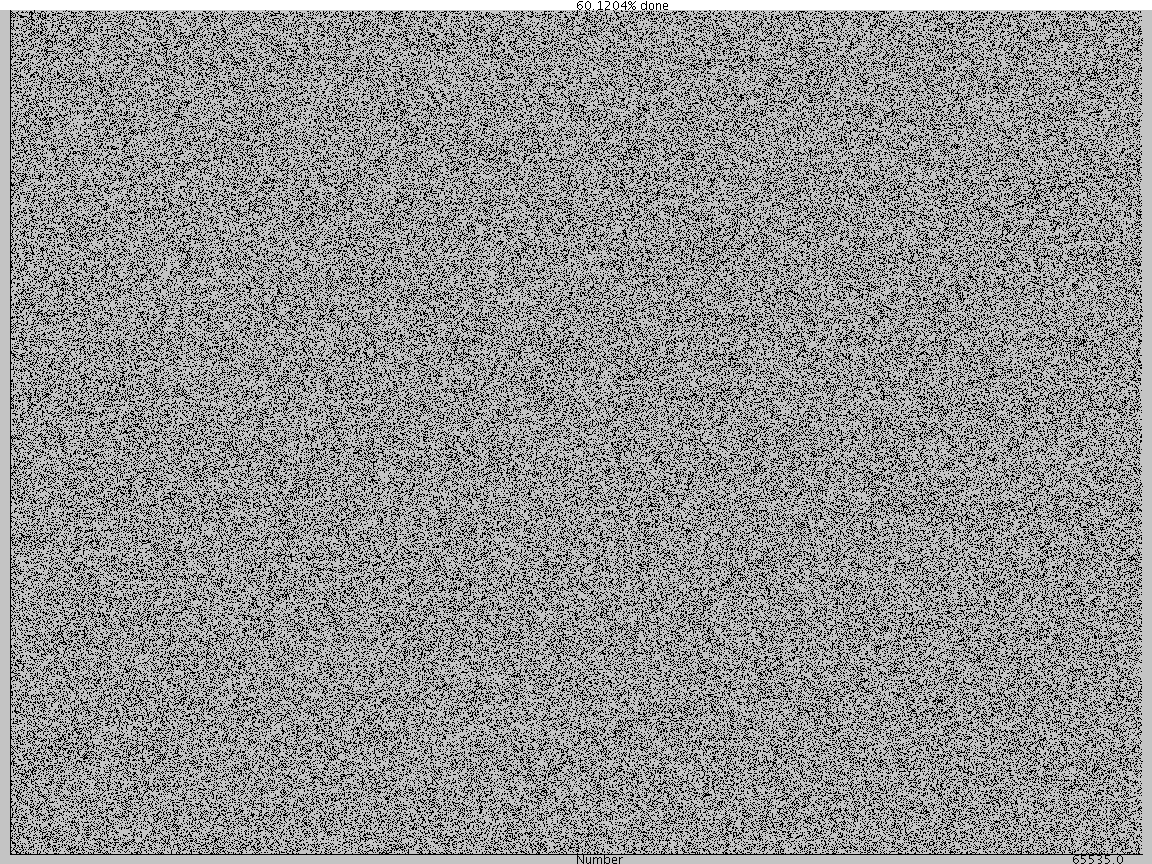
\includegraphics[width=10cm]{snapshot5.png}
   \caption{16-bit at 60\%}
   \label{Figure:figex}
\end{figure}
\begin{figure}[htbp]
   \centering
   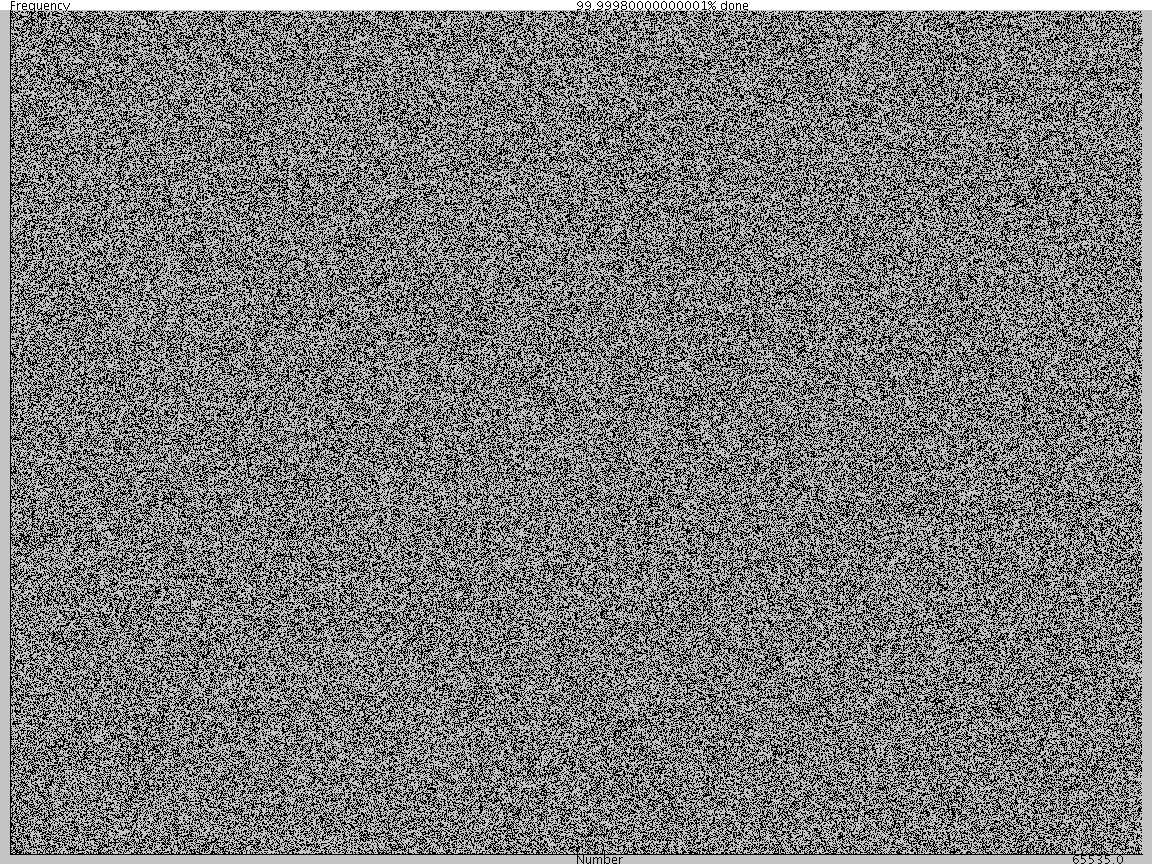
\includegraphics[width=10cm]{snapshot6.png}
   \caption{16-bit at 100\%}
   \label{Figure:figex}
\end{figure}
\newpage
\section{Conclusion}
Although generating truly random numbers can prove to be very difficult my program has definitely generated very good data. When I wanted to use the runs up test I found that the test is seriously flawed because the formula depends too much on the amount of numbers that were generated and thus increases exponentially. The dotplot graph proved to be a very useful tool in obtaining a understanding of how the numbers are generated and showed me that with my function the Tausworthe generator gives good numbers without depending on the seed that was chosen.
\section{References}
\begin{enumerate}
\item Law, Kelton
\emph{Simulation Modeling and Analysis} , pages 420-461.
\end{enumerate}
\end{document}
